\section{Finding 12 - SYN Flooding Attack}
\hrule\begin{table}[htb]
    \renewcommand{\arraystretch}{1.5}
    \begin{tabular*}{\textwidth}{|>{\columncolor{orange!15}}p{3cm}|p{17.2cm}|}
    \textbf{Finding} & \textbf{SYN Flooding Attack}\\
    Risk& Medium\\
    Category& Denial of Service\\
    Impact& The DUT is not accessible\\\\
    Description& The execution of a SYN Flooding Attack was accomplished with the following command: \newline
    hping3 -c 15000 -d 120 -S -w 64 -p 80 --flood --rand-source 172.16.0.29
    \newline
    This command sends 15000 packets with 120 bytes and a window size of 64 to port 80.
    \newline
    \newline
    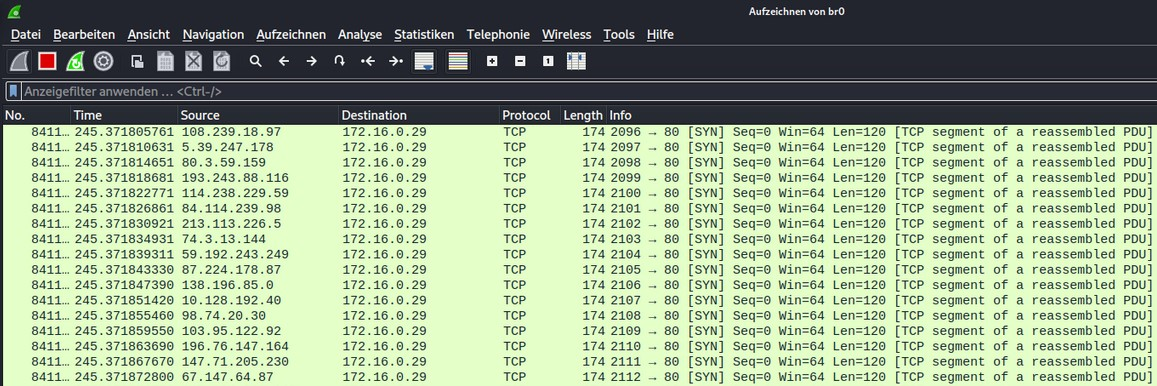
\includegraphics[width=0.85\textwidth]{wireshark_dos.jpg}
    \newline
    Illustrated in the graphic, wireshark captured the TCP SYN packages which were send to the DUT. After a couple of seconds it was not possible to access the server anymore.
	\\ 
	&\\
	&\\
	&\\
	&\\
	&\\
	&\\
	&\\
	&\\
    Recommendation& Possible countermeasures to SYN Flooding are intrusion prevention systems that monitor the network for suspicious behaviour or implementing SYN cookies to track incoming connection until the three-way handshake is completed.\\  
    \\\\
    \end{tabular*}
    \end{table}